\begin{center}
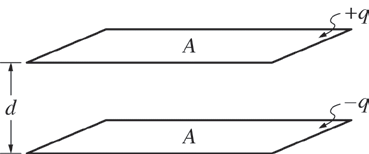
\includegraphics[scale=0.5]{images/img-008-020.png}
\end{center}

% Multiple Choice Question 26
\begin{questions}\setcounter{question}{25}\question
A parallel-plate capacitor of capacitance $C$ consists of two plates of area $A$ separated by distance $d$ as shown above. The upper and lower plates are given a net charge of $+q$ and $-q$, respectively. What is the electric field between the plates?

\begin{oneparchoices}
\choice Zero
\choice $\dfrac{C}{2 q d}$
\choice $\dfrac{C}{q d}$
\choice $\dfrac{2 q}{C d}$
\choice $\dfrac{q}{C d}$
\end{oneparchoices}\end{questions}

